\rhead{Deterministische endliche Automaten}
\section{Deterministische endliche Automaten\label{regulaer:dea}}
Ein endlicher Automat modelliert ein System, welches
in einer endlichen Zahl verschiedener Zustände sein kann.
Der Übergang zwischen den Zuständen geschieht deterministisch beim
Eintreffen neuer Daten.

Als Beispiel betrachten wir ein Drehkreuz an einem Skilift.
Es hat zwei mögliche Zustände: {\it  verriegelt} ($V$)
und  {\it entriegelt} ($E$).
Ausserdem gibt es zwei Inputs: {\tt Fahrkarte} ($F$)
und {\tt Drehen} ($D$).
Zu Beginn befindet sich das Drehkreuz in verriegeltem Zustand.
Wenn ein Skifahrer durch will, es zu drehen
versucht, ändert sich daran nichts.
Erst wenn er eine Fahrkarte einschiebt,
wird das Drehkreuz entriegelt.
Jetzt nützt es nichts, noch weitere
Fahrkarten einzuschieben, das Drehkreuz bleibt entriegelt.
Versucht der Skifahrer jetzt, das Drehkreuz zu drehen, wird es
ihn durchlassen, dabei aber wieder in den verriegelten Zustand übergehen.
Schematisch können wird das wie folgt darstellen:
\[
\entrymodifiers={++[o][F]}
\xymatrix{
*+\txt{} \ar[r]
	&{V}\ar@/^/[r]^{F} \ar@(ur,ul)_{D}
		&{E}\ar@/^/[l]^{D} \ar@(ur,ul)_{F}
}
\]
Wir sehen hier bereits eine Möglichkeit, Inputfolgen zu beobachten, 
aber es kann noch nicht entschieden werden, welche Inputs akzeptabel
sind.
Dazu müssen die einzelnen Zustände ausgezeichnet werden.
Zum Beispiel könnte man verlangen, dass nur Abläufe akzeptabel
sind, bei denen das Drehkreuz am Ende im verriegelten Zustand steht,
also nicht offen stehen bleibt.
Symbolisch bezeichnen wir dies durch einen Doppelkreis:
\[
\entrymodifiers={++[o][F]}
\xymatrix{
*+\txt{} \ar[r]
	&*++[o][F=]{V}\ar@/^/[r]^{F} \ar@(ur,ul)_{D}
		&{E}\ar@/^/[l]^{D} \ar@(ur,ul)_{F}
}
\]
Damit haben wir alle Elemente zusammen, die einen deterministischen
endlichen Automaten ausmachen.
\subsection{Definition\label{regulaer:definition-dea}}
\index{Automat!endlicher}%
\index{Automat!deterministischer endlicher}%
\index{DEA|see{deterministischer endlicher Automat}}%
Eine abstrakte Definition muss die Menge der erlaubten Inputs
festlegen, wir brauchen also ein Alphabet $\Sigma$.
Die Zustände bilden eine Menge.
Ausserdem müssen wir festlegen, in welchem Zustand
sich der Automat zu Beginn befindet und wie er auf ein Input-Zeichen
reagiert.
Dies wird erreicht durch die folgende Definition
\begin{definition}
Ein deterministischer endlicher Automat (DEA) ist ein Quintupel
$(Q,\Sigma,\delta, q_0,F)$ mit
\begin{compactenum}
\item $Q$ ist eine beliebige endliche Menge von Zuständen
\item $\Sigma$ ist eine endliche Menge, genannt das Alphabet.
\index{Übergangsfunktion!eines endlichen Automaten}%
\item $\delta\colon Q\times\Sigma\to Q$ heisst Übergangsfunktion
\index{Startzustand}%
\item $q_0\in Q$ heisst Startzustand
\index{Akzeptierzustand}%
\item $F\subset Q$ heisst die Menge der Akzeptierzustände.
\end{compactenum}
\end{definition}
Die Abbildung $\delta\colon Q\times \Sigma\to Q$ berechnet
aus einem Ausgangszustand $q\in Q$ und einem Input-Zeichen $a\in\Sigma$
einen neuen Zustand $\delta(q,a)\in Q$, in den der Automat durch
die Verarbeitung von $a$ übergeht.

\subsubsection{Gerichteter beschrifteter Graph eines DEA}
\index{Graph!gerichteter!beschrifteter!eines DEA}%
Eine Visualisierung ist häufig übersichtlicher.
Die Zustände von $Q$ werden durch Kreise dargestellt.
Die Übergangsfunktion wird durch mit Buchstaben des Alphabets $\Sigma$
angeschriebene Kreise symbolisiert.
Akzeptierzustände werden durch doppelte Kreise markiert.
Der Startzustand wird durch einen
Pfeil angezeigt, der nicht einen Zustand als Ausgangspunkt hat.

Damit haben wir einen gerichteten beschrifteten Graphen definiert.
Die Vertizes des Graphen sind die Zustände, also $V=Q$.
Vom Zustand $q$ aus verläuft eine mit $a\in\Sigma$ beschriftete
Kante zum Zustand $\delta(q,a)$, 
die Kantenmenge
ist also
\[
E=\{(q,\delta(q,a),a)\;|\; q\in Q\wedge a\in\Sigma\}.
\]
Darin nicht enthalten ist der Startzustand, den wir zwar auch als
Pfeil zeichnen, der aber nicht eine Kante des Graphen ist, weil
er nicht zwei Zustände verbindet.
Zusätzlich sind in diesem Graphen jedoch einzelne Zustände ausgezeichnet,
was wir in einem gewöhnlichen gerichteten Graphen nicht vorgesehen
haben.
Ein DEA ist also ein gerichteter beschrifteter Graph, aber nicht
nur.

Wichtig: von jedem Zustand aus gibt es genau einen Pfeil, der mit jedem möglichen
Zeichen des Alphabets angeschrieben sind.
Insbesondere kann man von jedem
Zustand aus mit jedem beliebigen Zeichen auf genau eine Art fortfahren.
\index{deterministisch}%
In diesem Sinne ist der Automat {\em deterministisch}.

\subsubsection{Beispiele}
\begin{beispiel}[\bf Drehkreuz]
Der Drehkreuz-DEA besteht aus den Elementen $Q=\{V,E\}$, $q_0=V$,
$F=\{V\}$, $\Sigma=\{F,D\}$.
Die Übergangsfunktion definiert zu jedem Zustand und jedem möglichen
Eingabewert, welcher zugehörige Zielwert erreicht wird:
\begin{center}
\begin{tabular}{|cc|c|}
\hline
$q$&$a$&$\delta(q,a)$\\
\hline
$V$&$D$&$V$\\
$V$&$F$&$E$\\
$E$&$D$&$V$\\
$E$&$F$&$E$\\
\hline
\end{tabular}
\end{center}
\end{beispiel}
\begin{beispiel}[\bf Gerade Binärzahlen]
Ein DEA, welcher erkennen kann, ob eine Bitfolge einer geraden Zahl entspricht.
Dieser DEA braucht zwei Zustände, denn eine Bitfolge, interpretiert
als Zahl, kann entweder gerade (Zustand $q_0$, Rest $0$ bei Teilung durch 2)
oder ungerade (Zustand $q_1$, Rest $1$) sein.
Die leere Bitfolge entspricht der Zahl $0$, also einer geraden Zahl.
Hinzufügen eines weiteren
Bits ändert den Zustand möglicherweise: hängt man eine $0$ an, entsteht
eine gerade Zahl, hänge man eine $1$ an, entsteht eine ungerade Zahl.
Wir haben also $\Sigma=\{\texttt{0},\texttt{1}\}$, $q_0$ als Startzustand,
$F=\{q_0\}$.
Die Übergangsfunktion ist
\begin{center}
\begin{tabular}{|cc|c|}
\hline
$q$&$a$&$\delta(q,a)$\\
\hline
$q_0$&$\texttt{0}$&$q_0$\\
$q_0$&$\texttt{1}$&$q_1$\\
$q_1$&$\texttt{0}$&$q_0$\\
$q_1$&$\texttt{1}$&$q_1$\\
\hline
\end{tabular}
\end{center}
Die graphische Form ist wiederum
\[
\entrymodifiers={++[o][F]}
\xymatrix{
*+\txt{}\ar[r]
	&*++[o][F=]{q_0} \ar@/^/[r]^{\texttt{1}} \ar@(ur,ul)_{\texttt{0}}
		&{q_1} \ar@/^/[l]^{\texttt{0}} \ar@(ur,ul)_{\texttt{1}}
}
\]
\end{beispiel}
\begin{beispiel}[\bf Dezimale Ganzzahlen]
Ein Automat, der Ganzzahlen ohne führende Nullen erkennt.
Das Alphabet besteht aus den Ziffern und dem optionalen Minus, also
\[
\Sigma=\{
{\tt 0},
{\tt 1},
{\tt 2},
{\tt 3},
{\tt 4},
{\tt 5},
{\tt 6},
{\tt 7},
{\tt 8},
{\tt 9},
{\tt -}
\}
\]
Eine ganze Zahl kann mit einem {\tt -} beginnen, darf
aber nicht mit einer {\tt 0} anfangen.
Danach dürfen beliebige
Ziffern folgen, aber kein {\tt -}.
Sobald ein {\tt -} eingegeben
wird, muss der Automat den Input als Illegal erkennen.
Offenbar gibt es also folgende Fälle: Zahl mit Minus, Zahl ohne Minus,
führende Null oder andere Illegalitäten.
Zusammen mit dem Startzustand sollten wir also mit vier Zuständen auskommen.
Sei $Q={q_0, m,p,e}$, dann wird das Zustandsdiagramm:
\begin{center}
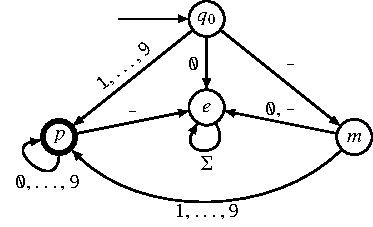
\includegraphics{3-regulaer/images/zahlen0.pdf}
\end{center}
\end{beispiel}
\begin{beispiel}[\bf Ganzzahlen, diesmal richtig]
Der eben gezeigte Automat ist insofern eine wörtliche Realisierung
der Anforderungen, dass er keine führende $0$ akzeptiert.
Allerdings
möchten wir in der Praxis auch eine einzelne $0$ akzeptieren können.
Dazu ist es nötig, den Automaten um einen Zustand zu erweitern:
\begin{center}
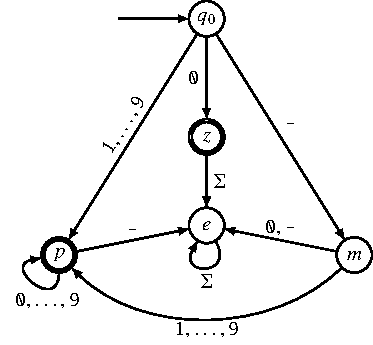
\includegraphics{3-regulaer/images/zahlen.pdf}
\end{center}
\end{beispiel}

\subsubsection{Tabellenform}
\index{Tabellenform eines DEA}%
Man kann alle Information eines DEA auch in einer einzigen Tabelle 
darstellen.
Die Zeilen werden mit den Zuständen angeschrieben,
die Spalten mit den Zeichen des Alphabetes.
Akzeptierzustände werden
mit {\tt /E} markiert, der Anfangszustand steht immer auf der ersten
Zeile.
Die oben betrachteten Beispiele haben folgende Tabellenform:

\begin{beispiel}[\bf Drehkreuz] $V$ ist Startzustand und gleichzeitig
Akzeptierzustand.

\begin{center}
\begin{tabular}{|c|cc|}
\hline
&$F$&$D$\\
\hline
$V{\tt /E}$&$E$&$V$\\
$E$&$E$&$V$\\
\hline
\end{tabular}
\end{center}

\end{beispiel}

\begin{beispiel}[\bf Gerade Zahlen]
Die Zustände $q_0$ und $q_1$ stehen für gerade und ungerade Zahlen:

\begin{center}
\begin{tabular}{|c|cc|}
\hline
&0&1\\
\hline
$q_0{\tt /E}$&$q_0$&$q_1$\\
$q_1$&$q_0$&$q_1$\\
\hline
\end{tabular}
\end{center}

\end{beispiel}

\begin{beispiel}[\bf Ganzzahl-Automat] Dieser Automat erkennt die $0$
nicht korrekt.

\begin{center}
\begin{tabular}{|c|ccccccccccc|}
\hline
&\tt 0&\tt 1&\tt 2&\tt 3&\tt 4&\tt 5&\tt 6&\tt 7&\tt 8&\tt 9&\tt -\\
\hline
$q_0$&$e$&$p$&$p$&$p$&$p$&$p$&$p$&$p$&$p$&$p$&$m$\\
$p{\tt /E}$&$p$&$p$&$p$&$p$&$p$&$p$&$p$&$p$&$p$&$p$&$e$\\
$m$&$e$&$p$&$p$&$p$&$p$&$p$&$p$&$p$&$p$&$p$&$e$\\
$e$&$e$&$e$&$e$&$e$&$e$&$e$&$e$&$e$&$e$&$e$&$e$\\
\hline
\end{tabular}
\end{center}

\end{beispiel}

\begin{beispiel}[\bf Ganzzahl-Automat mit $0$] Um die $0$ richtig zu erkennen,
wird ein zusätzlicher Zustand benötigt.

\begin{center}
\begin{tabular}{|c|ccccccccccc|}
\hline
&\tt 0&\tt 1&\tt 2&\tt 3&\tt 4&\tt 5&\tt 6&\tt 7&\tt 8&\tt 9&\tt -\\
\hline
$q_0$&$0$&$p$&$p$&$p$&$p$&$p$&$p$&$p$&$p$&$p$&$m$\\
$0{\tt /E}$&$e$&$e$&$e$&$e$&$e$&$e$&$e$&$e$&$e$&$e$&$e$\\
$p{\tt /E}$&$p$&$p$&$p$&$p$&$p$&$p$&$p$&$p$&$p$&$p$&$e$\\
$m$&$e$&$p$&$p$&$p$&$p$&$p$&$p$&$p$&$p$&$p$&$e$\\
$e$&$e$&$e$&$e$&$e$&$e$&$e$&$e$&$e$&$e$&$e$&$e$\\
\hline
\end{tabular}
\end{center}

\end{beispiel}

\subsection{Von einem DEA akzeptierte Sprache\label{regulaer:akzeptiertesprache}}
\index{akzeptierte Sprache eines DEA}%
Ein DEA definiert auf natürliche Weise eine Sprache: Sie besteht aus
allen Wörtern, die als Input für den DEA angewendet, diesen vom
Startzustand in einen Akzeptierzustand überführen.

\begin{definition}
Sei $A$ ein endlicher Automat, dann ist $L(A)$ die Sprache
\[
L(A)=\{w\in\Sigma^*\;|\; \text{$w$ überführt $A$ in einen Akzeptierzustand}\}
\]
\end{definition}

\begin{definition}
\label{regulaer:definition:regulaere-sprache}
\index{Sprache!reguläre}%
Eine Sprache heisst regulär, wenn es einen DEA gibt, der sie
akzeptiert.
\end{definition}

\subsubsection{Beispiele}
\begin{beispiel}[\bf Durch drei teilbare Zahlen] 
Man finde einen Automaten, der die durch drei teilbaren Zahlen in
Binärdarstellung akzeptiert.
Sei also $\Sigma=\{{\tt 0},{\tt 1}\}$,
$L=\{w\in\Sigma^*\;|\; \text{$w$ stellt eine durch drei teilbare Zahl dar}\}.$
Dabei soll das leere Wort für als $0$
interpretiert werden und damit auch als durch drei teilbar gelten.
Die Sprache $L$ ist regulär, weil sie
von folgendem Automaten akzeptiert wird:
\[
\entrymodifiers={++[o][F]}
\xymatrix{
*+\txt{} \ar[r]
	&*++[o][F=]{0} \ar@/^/[rr]^{\tt 1} \ar@(ur,ul)_{\tt 0}
		&*+\txt{}
			&{1} \ar@/^/[dl]^{\tt 0}  \ar@/^/[ll]^{\tt 1}
\\
*+\txt{}
	&*+\txt{}
		&2\ar@/^/[ur]^{\tt 0} \ar@(dl,ul)^{\tt 1}
}
\]
oder in Tabellenform
\begin{center}
\begin{tabular}{|c|cc|}
\hline
&\tt 0&\tt 1\\
\hline
0{\tt /E}&0&1\\
1        &2&0\\
2        &1&2\\
\hline
\end{tabular}
\end{center}
\end{beispiel}

\begin{beispiel}[\bf Wörter mit einer geraden Anzahl $a$]
Sei $\Sigma=\{{\tt a},{\tt b}\}$,
$L=\{w\in\Sigma^*\;|\; |w|_{\tt a}\equiv 0\mod 2\}$.
$L$ besteht aus den Wörtern, die  eine gerade Anzahl von {\tt a}s enthalten.
Diese Sprache ist regulär, weil sie von folgendem Automaten akzeptiert wird:
\[
\entrymodifiers={++[o][F]}
\xymatrix{
*+\txt{} \ar[r]
	&*++[o][F=]{0}\ar@/^/[r]^{\tt a} \ar@(dl,dr)_{\tt b}
		&1 \ar@/^/[l]^{\tt a} \ar@(dl,dr)_{\tt b}
}
\qedhere
\]
\end{beispiel}

\begin{beispiel}[\bf Bedingungen an einzelne Zeichen]
Finde einen Automaten, der die Sprache $L$ über dem Alphabet
$\Sigma=\{{\tt a},{\tt b}\}$ akzeptiert, deren Wörter mit 
einem {\tt a} beginnen und genau ein {\tt b} enthalten.
\[
\entrymodifiers={++[o][F]}
\xymatrix{
*+\txt{} \ar[r]
	&{q_0} \ar[r]^{\tt a} \ar[dr]^{\tt b}
		&{q_1} \ar@(ul,ur)^{\tt a} \ar[r]^{\tt b}
			&*++[o][F=]{q_2}\ar@(ul,ur)^{\tt a}  \ar[dl]^{\tt b}
\\
*+\txt{}
	&*+\txt{}
		&{e}\ar@(dl,dr)_{{\tt a},{\tt b}}
}
\]
\end{beispiel}

\subsection{Rekonstruktion des Automaten\label{regulaer:rekonstruktion}}
Wenn eine Sprache regulär ist, dann muss es einen DEA geben, der
diese Sprache erkennt.
Doch wie findet man aus der Sprache, also aus der Menge $L$, diesen DEA?

Nehmen wir an, der DEA sei schon bekannt, und versuchen wir,
die Zustände zu charakterisieren.
Befindet sich ein Automat im Zustand $q$, dann kann durch zusätzlichen
Input $w_e$ ein akzeptables Wort entstehen.
Sei also $L(q)$ die Menge der Wörter, mit deren Hilfe man vom Zustand $q$
aus einen Akzeptierzustand erreichen kann.
Wenn man mit einem Wort $w_a$ den Zustand $q$ erreicht, dann ist $L(q)$
offenbar auch
\[
L(q)=\{ w_e\;|\; w_aw_e \in L\}= L(w_a)
\]
Die Mengen $L(w)$ können also ganz allein aus der Kenntnis der
Sprache bestimmt werden, die $L(q)$ sind nicht mehr nötig.

Wir zeigen jetzt, dass wir mit den Mengen $L(w)$ als Zuständen einen
DEA bauen können, der genau die Sprache $L$ akzeptiert.
Wir setzen als für die Menge der Zustände 
\[
Q=\{L(w)\;|\;w\in\Sigma^*\}.
\]

Ein Wort muss offenbar genau dann akzeptiert werden, wenn
man es ans leere Wort anhängen kann und damit zu einem Akzeptierzustand
kommt, also $L=L(\varepsilon)$.
Dies ist der Anfangszustand des Automaten, also
\[
q_0=L.
\]

Die Übergangsfunktion $\delta$ führt die Menge $L(w)$ bei Input
$a$ in die Menge $L(wa)$ über, also
\[
\delta \colon Q\times\Sigma\to Q:(L(w),a)\mapsto L(wa).
\]

Akzeptierzustande sind offenbar diejenigen $L(w)$, von denen
aus man nicht mehr weiter gehen muss, um einen Akzeptierzustand
zu erreichen, also jene $L(w)$ die das leere Wort enthalten:
\[
F=\{L(w)\;|\;\varepsilon\in L(w)\}.
\]

Wir nennen den eben konstruierten Automaten $A$.
Jetzt müssen wir nur noch zeigen, dass dieser Automat genau die
Wörter in $L$ akzeptiert.
Sei das Wort $w\in L$ zusammengesetzt aus den
Zeichen $a_1,a_2,\dots,a_n$, also $w=a_1a_2\dots a_n$.
Dann führt der Input $w$ den Anfangszustand $L$ schrittweise über in
\[
L(a_1)\to L(a_1a_2)\to L(a_1a_2a_3)\to \dots \to L(a_1a_2\dots a_n),
\]
da letzterer das leere Wort enthält, ist er ein Akzeptierzustand.
Ein Wort in $L$ wird also automatisch vom Automaten $A$ akzeptiert.

Jetzt müssen wir noch nachweisen, dass ein von $A$ akzeptiertes Wort $w$
auch in $L$ drin liegt.
Dass $A$ das Wort $w$ akzeptiert besagt, dass $\varepsilon \in L(w)$.
Das ist aber gleichbedeutend damit, dass $w\in L$.
Damit ist alles bewiesen und wir den haben folgenden Satz.

\begin{satz}[Myhill-Nerode]\label{satz_dea_aus_sprache}
\index{Myhill-Nerode!Satz von}%
Ist $L$ eine reguläre Sprache, dann wird $L$ von dem 
endlichen Automaten $A=(Q,\Sigma,\delta,q_0,F)$ akzeptiert mit
\begin{align*}
Q&=\{L(w)\;|\;w\in\Sigma^*\}\\
q_0&=L\\
F&=\{q\in Q\;|\; \varepsilon\in q\}\\
\delta&\colon Q\times \Sigma\to Q:(L(w),a)\mapsto L(wa)
\end{align*}
\end{satz}

\subsubsection{Beispiel}
Wir rekonstruieren den Automaten für die folgende Sprache über
$\Sigma=\{{\tt a},{\tt b}\}$:
\[
L=\{w\in \Sigma^*\;|\; |w|_{\tt a}\equiv 0\mod 2\}.
\]
Dazu müssen wir die Menge der möglichen $L(w)$ ermitteln:
\begin{center}
\begin{tabular}{|c|l|}
\hline
$w$&$L(w)$\\
\hline
$\varepsilon$&$L$\\
{\tt a}&$L({\tt a})=\{w\in\Sigma^*\;|\; \text{$|w|_a$ ungerade}\}$\\
{\tt b}&$L({\tt b})=\{w\in\Sigma^*\;|\; \text{$|w|_a$ gerade}\}=L$\\
$|w|_{\tt a}$ ungerade&$L({\tt a})$\\
$|w|_{\tt a}$ gerade&$L$\\
\hline
\end{tabular}
\end{center}
Offenbar gibt es also genau die zwei Zustände $L$ und $L'=L({\tt a})$.
Ein Zeichen {\tt a} führt $L$ in $L({\tt a})$ über und umgekehrt,
das Zeichen {\tt b} ändert den Zustand nicht:
\[
\entrymodifiers={++[o][F]}
\xymatrix{
*+\txt{} \ar[r]
	&*++[o][F=]{L}\ar@/^/[r]^{\tt a} \ar@(ul,ur)^{\tt b}
		&{L'} \ar@/^/[l]^{\tt a} \ar@(ul,ur)^{\tt b}
}
\]
Dieser Automat ist identisch mit dem früher gefundenen.

Mit dem Satz von Myhill-Nerode erhalten wir damit auch einen Satz,
der zu entscheiden erlaubt, ob eine Sprache regulär ist.

\begin{satz}
Sei $L$ eine Sprache über $\Sigma$ und $L(w)=\{ v\in\Sigma^*\;|\; wv\in L\}$.
Falls die Menge 
\[
\{L(w)\;|\; w\in\Sigma^*\}
\]
endlich ist, ist $L$ regulär.
Falls sie unendlich ist, kann $L$ nicht regulär sein.
\end{satz}

Als Anwendung dieses Satzes zeigen wir, dass die Sprache
$\{ \texttt{0}^n\texttt{1}^n \;|\; n\in\mathbb N\}$ über
$\Sigma=\{\texttt{0},\texttt{1}\}$
nicht regulär ist.
Wir müssen also die Mengen $L(w)$ für alle denkbaren Wörter $w\in\Sigma^*$
ermitteln.
Dazu erstellen wir die folgende Tabelle:
\begin{center}
\begin{tabular}{|>{$}c<{$}|>{$}c<{$}|}
\hline
w                       &L(w)\\
\hline
\varepsilon             &L\\
\texttt{1}              &\emptyset\\
\texttt{1}^n            &\emptyset\\
\texttt{0}              &\{\texttt{0}^n\texttt{1}^{n+1}\;|\; n\in\mathbb N\}\\
\texttt{0}^2            &\{\texttt{0}^n\texttt{1}^{n+2}\;|\; n\in\mathbb N\}\\
\texttt{0}^k            &\{\texttt{0}^n\texttt{1}^{n+k}\;|\; n\in\mathbb N\}\\
\texttt{0}^k\texttt{1}^l&\{\texttt{1}^{k-l}\}$ falls $k\ge l\\
\texttt{0}^k\texttt{1}^l&\text{$\emptyset$ falls $k<l$}\\
\hline
\end{tabular}
\end{center}
An den Zeilen vier bis sieben kann man ablesen, dass es unendlich
viele verschiedene Mengen $L(w)$ gibt, somit kann $L$ nicht von
einem endlichen Automaten erkannt werden.

\subsection{Minimaler Automat\label{regulaer:minimalautomat}}
\index{Automat!minimaler}%
Zwei endliche Automaten können völlig verschieden aussehen,
und trotzdem die gleiche Sprache akzeptieren.
Kann man auf einfache
Art herausfinden, ob zwei endliche Automaten die gleiche Sprache
akzeptieren?

Gäbe es für einen Automaten die Möglichkeit, ihn in eine Standardform
zu bringen, so könnte man diese für einen solchen Vergleich verwenden.
Zunächst müsste man beide Automaten in die Standardform bringen.
Wenn die Standardformen übereinstimmen, akzeptieren sie die gleiche Sprache.

Eine Standardform eines Automaten können wir über die Konstruktion
aus Satz \ref{satz_dea_aus_sprache} ermitteln: Zu einem Automaten
$A$ ermitteln wir zunächst die Sprache $L=L(A)$, für die wir dann
den Automaten aus Satz \ref{satz_dea_aus_sprache} bilden.

\begin{satz}[Minimalautomat]\label{satz_minimalautomat}
Sei $A$ ein DEA und $A'$ der DEA, der nach
Satz \ref{satz_dea_aus_sprache} gebildet wurde.
Dann gibt es eine surjektive Abbildung der Zustände $f\colon Q\to Q'$, so dass
\begin{compactenum}
\item $f(q_0)=q_0'=L$
\item $\delta'(f(q),a)=f(\delta(q,a))$
\item $q\in F\Rightarrow f(q)\in F'$
\end{compactenum}
Insbesondere ist $A'$ der kleinste aller Automaten, der die Sprache
$L$ akzeptieren kann.
\end{satz}

\begin{proof}[Beweis]
Jedes Wort $w\in\Sigma^*$ führt den Automaten $A$ aus dem
Anfangszustand in einen Zustand $q\in Q$.
Führen zwei Wörter $w_1$ und $w_2$ den DEA $A$ in den gleichen Zustand $q$,
werden von dort aus die gleichen Wörter akzeptiert, d.\,h.~$L(w_1)=L(w_2)$.
Die Abbildung
\[
f\colon Q\to Q': q\mapsto L(w)
\]
ist also unabhängig von dem Wort $w$, mit welchem man den Zustand $q$
erreicht hat.

Jetzt muss gezeigt werden, dass $f$ die genannten Eigenschaften hat:
\begin{compactenum}
\item
$\varepsilon$ führt $A$ in den Anfangszustand über, also
$f(q_0)=L(\varepsilon)=L=q_0'$.
\item Falls $w$ den DEA in den Zustand $q$ führt, führt das Wort
$wa$ den DEA in den Zustand, den man von $q$ mit Input $a$ erreicht.
Also ist
\[
\delta'(f(q),a)=\delta'(L(w), a)=L(wa)=f(\delta(q,a))
\]
\item Sei $q\in F$ und sei $w$ ein Wort, welches den DEA in den Zustand 
$q$ führt.
Dann ist $f(q)=L(w)$, da aber $q$ ein Akzeptierzustand ist,
ist $\varepsilon\in L(w)$, $f(q)$ ist also ein Akzeptierzustand von
$A'$.
\qedhere
\end{compactenum}
\end{proof}

Die Bestimmung des Automaten über den Satz \ref{satz_dea_aus_sprache}
ist eher umständlich.
Der Satz \ref{satz_minimalautomat} zeigt
aber auch, dass wir einfach nach einem DEA suchen müssen, in dem
möglichst viele Zustände zusammengelegt worden sind, bis sich die
Anzahl der Zustände nicht mehr weiter verringern lässt.

Wir müssen also herausfinden, welche Zustände man zusammenlegen
kann.
Das sind natürlich genau diejenigen, die das gleiche $L(q)$
haben.
\index{aquivalent Zustande@äquivalent!Zustände}%
Statt herauszufinden, welche Zustände in diesem Sinne äquivalent
sind, könnte man auch herauszufinden versuchen, welche nicht äquivalent
sind.
Als Beispiel nehmen wir den folgenden Automaten
\[
\entrymodifiers={++[o][F]}
\xymatrix{
*+\txt{}
	&*+\txt{}
		&{z_1}\ar@/_/[dd]_{0} \ar[dr]^{1}
\\
*+\txt{} \ar[r]
	&{z_0}\ar[ur]^{0} \ar[dr]_1
		&*+\txt{}
			&*++[o][F=]{z_3}\ar@(ur,dr)^{0,1}
\\
*+\txt{}
	&*+\txt{}
		&{z_2} \ar@/_/[uu]_{0} \ar[ur]_{1}
}
\]
Von den zwei Zuständen $z_1$ und $z_2$ aus kann man genau die gleichen
akzeptierten Wörter bilden, also $L(z_1)=L(z_2)$, man müsste diese
also zusammenlegen können.

\index{Algorithmus!für den Minimalautomaten}%
\subsubsection{Algorithmus für den Minimalautomaten
\label{algorithmus:minimalautomat}}
Um solche Zustände zu finden, erstellen wir jetzt eine Tabelle, in der
wir aufzeichnen, welche Zustände äquivalent sind oder auch nicht.
Äquivalente Zustände markieren wir mit dem Zeichen $\equiv$, nicht
äquivalente mit einem Kreuz $\times$.
Zunächst wissen wir nur, dass jeder Zustand zu sich selbst äquivalent
ist, also
\begin{center}
\begin{tabular}{ccccc}
     &$z_0$   &$z_1$   &$z_2$   &$z_3$   \\
$z_0$&$\equiv$&        &        &        \\
$z_1$&        &$\equiv$&        &        \\
$z_2$&        &        &$\equiv$&        \\
$z_3$&        &        &        &$\equiv$
\end{tabular}
\end{center}
Zwei Zustände können nicht äquivalent sein, wenn der eine
ein Akzeptierzustand ist, der andere hingegen nicht, wir markieren
also alle solchen Paare mit einem $\times$, füllen aber nur den Teil unterhalb der
Diagonalen aus.
\begin{center}
\begin{tabular}{ccccc}
     &$z_0$   &$z_1$   &$z_2$   &$z_3$   \\
$z_0$&$\equiv$&        &        &        \\
$z_1$&        &$\equiv$&        &        \\
$z_2$&        &        &$\equiv$&        \\
$z_3$&$\times$&$\times$&$\times$&$\equiv$
\end{tabular}
\end{center}
Falls man von den Zuständen $p$ und $q$ mit einem Übergang
ein bereits mit $\times$ markiertes Feld erreichen kann, können die
Zustände $p$ und $q$ nicht äquivalent sein, man muss also auch das
Feld $(p,q)$ mit $\times$ markieren.
Vom Paar $(z_0,z_1)$ aus kann man zum Beispiel mit einer $1$ das
Paar $(z_2,z_3)$ erreichen, welche als nicht äquivalent bekannt
sind.
Ebenso kann man von $(z_0,z_2)$ mit einer $1$ das Paar
$(z_2,z_3)$ erreichen.
So findet man die Tabelle
\begin{center}
\begin{tabular}{ccccc}
     &$z_0$   &$z_1$   &$z_2$   &$z_3$   \\
$z_0$&$\equiv$&        &        &        \\
$z_1$&$\times$&$\equiv$&        &        \\
$z_2$&$\times$&        &$\equiv$&        \\
$z_3$&$\times$&$\times$&$\times$&$\equiv$
\end{tabular}
\end{center}
Das verbleibende Paar $(z_1,z_2)$ wird aber immer in $(z_1,z_2)$ 
oder $(z_3,z_3)$ übergeführt, von beiden Paare können wir nicht
schliessen, dass sie nicht äquivalent sind, also müssen sie äquivalent
sein:
\begin{center}
\begin{tabular}{ccccc}
     &$z_0$   &$z_1$   &$z_2$   &$z_3$   \\
$z_0$&$\equiv$&        &        &        \\
$z_1$&$\times$&$\equiv$&        &        \\
$z_2$&$\times$&$\equiv$&$\equiv$&        \\
$z_3$&$\times$&$\times$&$\times$&$\equiv$
\end{tabular}
\end{center}
Man kann also die beiden Zustände $z_1$ und $z_2$ zusammenlegen,
und erhält den minimalen Automaten:
\[
\entrymodifiers={++[o][F]}
\xymatrix{
*+\txt{} \ar[r]
	&{z_0}\ar[r]^{0,1} 
		&{z_{1,2}}\ar@(ur,ul)_{0}\ar[r]^1
			&*++[o][F=]{z_3}\ar@(ur,dr)^{0,1}
}
\]

Der Vergleich von zwei deterministischen endlichen Automaten ist zwar
mit Hilfe des Minimalautomaten möglich, dies ist jedoch nicht der
bestmögliche Algorithmus.
Ein Algorithmus mit linearer Laufzeit wurde von Hopcroft und Karp
angegeben.
\begin{figure}
\begin{center}
\includegraphics{images/reg-6.pdf}
\end{center}
\caption{Pumping Lemma: Zerlegung eines Wortes $w$ in drei Teile
$w=xyz$.\label{regular:pumpinglemma-graph}}
\end{figure}

\subsection{Pumping Lemma für reguläre Sprachen\label{regulaer:pumpinglemma}}
\index{Pumping Lemma!für reguläre Sprachen}%
Der Satz~\ref{satz_dea_aus_sprache} zeigt, wie man zu einer regulären Sprache
einen endlichen Automaten finden kann.
Als Nebeneffekt kann man daraus oft auch ableiten, ob eine Sprache regulär
ist.
Wenn allerdings die Zahl der Zustände sehr gross ist, kann man beim
Auflisten der Zustände nicht unterscheiden, ob man einfach noch etwas
mehr Geduld haben muss, bis man alle Zustände gefunden hat, oder ob
es tatsächlich unendlich viele verschiedene Mengen unter den $L(w)$
gibt.
Wir brauchen daher eine Methode, mit der man die Frage nach der
Regularität entscheiden können, ohne auf eine Auflistung aller
nötigen Zustände angewiesen zu sein.

Eine reguläre Sprache wird von einem DEA akzeptiert.
Dadurch wird die Struktur der Wörter eingeschränkt.
Ein Wort $w$ beschreibt
einen Pfad durch den gerichteten beschriftenten Graphen des DEA
(Abbildung~\ref{regular:pumpinglemma-graph}).
Wenn das Wort länger ist als die Anzahl der Zustände, dann muss
mindestens ein Zustand mehrmals vorkommen.
Wir können sogar
sagen, dass die erste solche Wiederholung innerhalb der ersten
$N = |Q|$ Zeichen des Wortes $w$ auftreten muss.
Sei $x$ das Wort,
das den Zustand in den ersten wiederholten Zustand $q$ führt.
Sei $y$ das kürzeste Wort, welches von $q$ wieder zu $q$ führt und
$z$ der Rest, also $w=xyz$.
Dann können wir die Schleife $y$
auch mehrmals wiederholen und immer ein Wort erhalten welches
vom Anfangszustand über den Zustand $q$ (evlt.~mehrmals) zu einem
Endzustand führt.
Die Wörter $xy^kz$ werden also alle auch von dem Automaten akzeptiert.
Damit haben wir folgendes bewiesen:
\begin{satz}[Pumping Lemma für reguläre Sprachen]
\index{pumping length!für reguläre Sprachen}%
Ist $L$ eine reguläre Sprache, dann gibt es eine Zahl $N$, die Pumping Length, so dass
jedes Wort $w\in L$ mit $|w|\ge N$ in drei Teile
$w=xyz$ zerlegt werden kann, so dass
\begin{compactenum}
\item $|y| > 0$
\item $|xy|\le N$
\item $xy^kz\in L\quad\forall k\ge 0$
\end{compactenum}
\end{satz}

Das Pumping Lemma dient in erster Linie dazu, von einer Sprache
nachzuweisen, dass sie nicht regulär ist.
Dazu nimmt man an, dass die Sprache regulär ist, für sie also die Aussage
des Pumping Lemma gilt.
Dann leitet man daraus einen Widerspruch ab.


\begin{beispiel}[\bf Eine nicht reguläre Sprache]
Wir führen dies an dem Beispiel der Sprache $L=\{0^n1^n|n\ge 0\}$
durch, welche wir bereits als nicht regulär erkannt haben.
Wir nehmen jetzt also an, dass $L$ regulär sei.
Dann gibt es nach dem Pumping Lemma eine Zahl $N$, so dass Wörter mit
mindestens dieser Länge interessante Eigenschaften haben.
Wir wählen das Wort
\[
0^N1^N\in L
\]
Nach dem Pumping Lemma muss $w$ in drei Teile aufgeteilt werden können
(Abbildung~\ref{plimage}),
$w=xyz$,
wovon die ersten beiden Teile $x$ und $y$ zusammen eine Länge $\le N$
haben, also aus lauter Nullen bestehen müssen.
Der Teil $y$ muss mindestens eine Null enthalten.
Wenn man jetzt $xy^kz$ bildet, vermehrt man die Zahl der Nullen,
nicht aber die Zahl der Einsen, man erhält also ein Wort, welches
mehr Nullen als Einsen enthält.
Das Pumping Lemma sagt, dass $xy^kz\in L$, aber die Definition von $L$ sagt,
dass ein Wort in $L$ gleich viele Nullen wie Einsen haben muss, also
$xy^kz\not\in L$ für $k>1$.
Dieser Widerspruch zeigt, dass die ursprüngliche
Annahme, $L$ sei regulär gewesen, nicht haltbar ist.
Also ist die Sprache nicht regulär.
\begin{figure}
\begin{center}
\begin{tabular}{l}
\includegraphics{images/pl-2.pdf}\\
\includegraphics{images/pl-1.pdf}\\
\includegraphics{images/pl-3.pdf}\\
\includegraphics{images/pl-4.pdf}
\end{tabular}
\end{center}
\caption{Anwendung des Pumping-Lemmas.
Ein genügend langes Wort
der Sprache $w=0^N1^N$ kann nach dem Pumping Lemma in $w=xyz$ 
zerlegt werden (2.~Zeile).
Das Pumping Lemma verspricht, dass
abgepumpte Wörter (3.~Zeile) und aufgepumpte Wörter (4.~Zeile)
auch zur Sprache gehören sollen, tun sie aber nicht.
\label{plimage}}
\end{figure}
\end{beispiel}

\subsubsection{Beispiel}
\index{Palindrom}%
Ein Palindrom ist ein Wort, welches ``vorwärts'' und ``rückwärts''
gleich lautet.
Zum Beispiel {\tt otto}, {\tt anna}, {\tt reittier} oder der
Klassiker
\begin{center}
{\tt erika feuert nur untreue fakire}
\end{center}
Formal können wir das so beschreiben: ist $w=a_1a_2\dots a_n\in\Sigma^*$
ein Wort, dann sei $w^t=a_na_{n-1}\dots a_2a_1$ das ``rückwärts
geschriebene Wort:
\[
{\tt esel}^t={\tt lese},\quad {\tt reliefpfeiler}^t={\tt reliefpfeiler}.
\]
Palindrome sind offenbar Wörter, die sich bei Anwendung der
$\mathstrut^t$-Operation nicht ändern: $w^t=w$.
Die Menge der Palindrome
ist natürlich eine Sprache $L=\{w\in\Sigma^*\;|\;w^t=w\}$.

Wir zeigen jetzt, dass die Menge der Palindrome keine reguläre Sprache ist.
Dazu verwenden wir das Pumping-Lemma, wir nehmen also an, die Sprache
sei regulär und führen dies mit dem Pumping Lemma zu einem Widerspruch:
\begin{compactenum}
\item Das Pumping Lemma verspricht, dass es eine Zahl $N$ gibt, die
Pumping Length.
\item Wir bilden jetzt das Wort $0^N10^N$.
Dieses Wort ist ein Palindrom,
also in $L$.
\item Das Pumping Lemma garantiert jetzt eine Zerlegung des Wortes
in drei Teile $xyz$, mit den Eigenschaften $|xy|\le N$, $|y|\ge 1$ und
$xy^kz\in L\forall k\in\mathbb N$.
\item Wir prüfen dies nach für $k=2$ (Abbildung~\ref{regular:pl-palindrome}).
\begin{figure}
\centering
\includegraphics{images/palindrom-1.pdf}
\caption{Anwendung des Pumping-Lemmas auf die Sprache der Palindrome
\label{regular:pl-palindrome}}
\end{figure}
Da $|xy|\le N$, bestehen sowohl $x$ als auch $y$ aus lauter Nullen.
Die $1$ befindet sich im Teil $z$.
Das Wort $xyyz$ hat daher $N+|y|$ Nullen vor der $1$, aber nur $N$ Nullen
nach der $1$, ist also kein Palindrom mehr.
Es ist also $xy^2z\not\in L$,
im Widerspruch zur Ausssage des Pumping Lemma (vorangegangener Schritt).
\end{compactenum}
Der Widerspruch zeigt jetzt, dass die Annahme, $L$ sei regulär, nicht
haltbar ist, $L$ ist also nicht regulär.

\subsubsection{Eine pumpbare aber nicht reguläre Sprache}
Das Pumping Lemma wird dazu verwendet nachzuweisen, dass eine Sprache
nicht regulär ist.
Dabei verwendet man, dass eine reguläre Sprache immer die Pumpeigenschaft
hat: lange Wörter lassen sich aufpumpen.
Das Pumping Lemma erlaubt aber die umgekehrte Schlussfolgerung nicht.
Eine Sprache mit der Pump-Eigenschaft ist nicht notwendigerweise auch
regulär, wie das nachfolgende Beispiel illustriert.

Wir betrachten dazu die Sprache
\[
L= \{ \texttt{a}^i\texttt{b}^j\texttt{c}^k\;|\; i=0\vee j=k\}.
\]
Die Sprache wird etwas leichter verständlich, wenn man sie in zwei 
disjunkte Teilsprachen
\(
L= L_1\cup L_2
\)
zerlegt mit
\begin{align*}
L_1
&=
\{\texttt{b}^j\texttt{c}^k\;|\; j,k\ge 0\}
\\
L_2
&=
\{\texttt{a}^i\texttt{b}^n\texttt{c}^n\;|\; i> 0\wedge n\ge 0\}.
\end{align*}
Die Sprache $L_1$ ist sicher regulär, man kann sie mit dem endlichen
Automaten
\begin{center}
\begin{tikzpicture}[>=latex,thick]
\coordinate (q0) at (0,0);
\coordinate (q1) at (2,0);
\coordinate (e)  at (4,0);
\draw (q0) circle[radius=0.3];
\draw (q0) circle[radius=0.35];
\node at (q0) {$q_0$};
\draw (q1) circle[radius=0.3];
\draw (q1) circle[radius=0.35];
\node at (q1) {$q_1$};
\draw (e) circle[radius=0.35];
\node at (e) {$e$};
\draw[->,shorten >= 0.35cm,shorten <= 0.35cm] (-2,0) -- (q0);
\draw[->,shorten >= 0.35cm,shorten <= 0.35cm] (q0) -- (q1);
\draw[->,shorten >= 0.35cm,shorten <= 0.35cm] (q1) -- (e);
\draw[->,shorten >= 0.35cm,shorten <= 0.35cm] (q0) to[out=60,in=120,distance=1.5cm] (q0);
\draw[->,shorten >= 0.35cm,shorten <= 0.35cm] (q1) to[out=60,in=120,distance=1.5cm] (q1);
\draw[->,shorten >= 0.35cm,shorten <= 0.35cm] (e) to[out=30,in=-30,distance=1.5cm] (e);
\node at ($0.5*(q0)+0.5*(q1)$) [above] {\texttt{b}};
\node at ($(q0)+(0,1)$) [above] {\texttt{a}};
\node at ($(q1)+(0,1)$) [above] {\texttt{b}};
\node at ($0.5*(q1)+0.5*(e)$) [above] {\texttt{a}};
\node at ($(e)+(1,0)$) [right] {\texttt{a},\texttt{b}};
\end{tikzpicture}
\end{center}
akzeptieren.
Die Teilsprache $L_2$ ist aber nicht regulär.
Mit dem Satz von Myhill-Nerode kann man ganz ähnlich wie bei der Sprache
$\{\texttt{0}^n\texttt{1}^n\;|\;n\ge 0\}$ nachweisen, dass es dafür
unendlich viele Zustände braucht.

Trotzdem hat die Sprache $L$ die Pumpeigenschaft.
In der Teilsprache $L_1$ ist dies klar, die Pumpeigenschaft folgt hier,
weil $L_1$ regulär ist aus dem Pumping Lemma.
Man kann aber auch direkt sehen, dass das erste Zeichen eines Wortes
immer aufgepumpt werden kann, die Pumpeigenschaft ist also sogar mit
Pumping Length $N=1$ erfüllt.

In der Teilsprache $L_2$ beginnt ein Wort immer mit dem Zeichen
\texttt{a}.
Dieses Zeichen kann beliebig vervielfacht werden, solange man die
nachfolgenden \texttt{b} und \texttt{c} nicht stört.
Damit hat auch $L_2$ die Pumpeigenschaft für $L_2$.
Somit kann in jedem Wort in $L$ mit mindestens einem Zeichen das erste
Zeichen beliebig aufgumpt werden, ohne dass das Wort dadurch aus der
Sprache herausfällt.
Die Sprache $L$ hat also die Pumpeigenschaft, ohne dass sie regulär ist.




